% =============================================================================
%  Institutional Profiles Under a Common Prudential Framework:
%  Evidence from Brazilian Credit Cooperatives and Banks
%  ICA CCR 2026 full submission
%
%  Tables come from tables/*.tex, generated by make_tables.py from results/*.txt.
%  Figures come from figures/. Do not transcribe numbers by hand.
%
%  TODO BEFORE SUBMISSION
%   [ ] award category below the title
%   [ ] author block (currently anonymised)
%   [ ] references.bib: entries marked VERIFY in the .bib need a
%       publisher-page check of volume/pages before submission
% =============================================================================
\documentclass[11pt,a4paper]{article}
\usepackage[utf8]{inputenc}
\usepackage[T1]{fontenc}
\usepackage{lmodern}
\usepackage[margin=1in]{geometry}
\usepackage{booktabs}
\usepackage{graphicx}
\usepackage{amsmath}
\usepackage{threeparttable}
\usepackage[hidelinks]{hyperref}
\usepackage[round]{natbib}
\usepackage{setspace}
\onehalfspacing

\title{\textbf{Institutional Profiles Under a Common Prudential Framework:}\\[0.3em]
\large Evidence from Brazilian Credit Cooperatives and Banks}
\author{[Author names withheld for review]}
\date{}

\begin{document}
\maketitle
\vspace{-2em}
\begin{center}
\textit{Award category:} [INSERT CATEGORY]
\end{center}

\begin{abstract}
\noindent In Brazil, a credit cooperative that grows past a size threshold computes
capital, leverage and risk under the same rules as a commercial bank. We use this setting
to ask whether the cooperative form still displays distinct balance-sheet characteristics
under equal regulation. The sample is every institution under the full prudential
methodology from 2017 to 2024: 130 credit cooperatives and 144 banks. At comparable size,
cooperatives lend more of their assets, earn more on them, spend less to do so, and have
steadier returns. They also hold less regulatory capital on average, although the gap
comes from a group of highly capitalised banks that has no cooperative counterpart. Among
thinly capitalised institutions, where supervisors look first, cooperatives hold more
capital than banks while provisioning at least as much. It is often claimed that
cooperatives provision less and earn narrower margins. This does not hold once the
comparison group is restricted to banks; the broad regulatory population contains nearly
two hundred institutions that neither lend nor take deposits. A prudential benchmark
calibrated on the average institution therefore describes cooperatives poorly, since they
do not occupy the part of the distribution that average is drawn from.

\medskip
\noindent\textbf{Keywords:} credit cooperatives; prudential regulation; Basel;
proportionality; Brazil.\\
\textbf{JEL:} G21, G28, P13.
\end{abstract}

% quebrei a pagina pra introducao comecar sozinha
\newpage

% =============================================================================
\section{Background}
%\section{Introduction}
% =============================================================================

Prudential regulation has converged on a common template. Basel III supplies the
architecture for capital, leverage and risk measurement, and national supervisors adapt
it locally \citep{bcbs2011}. Brazil sorts authorised institutions into five segments for
the proportional application of prudential rules \citep{cmn4553};
Figure~\ref{fig:regulatory} shows how the two populations divide between the
methodologies over our window. Segments 1 to 4 apply the full methodology. Segment~5
comprises institutions below 0.1~percent of GDP in size that use the optional simplified
method of computing minimum capital \citep{cmn4606}; commercial, multiple, investment and
exchange banks are excluded from it whatever their size. Membership of S5 therefore follows
from the choice of methodology, and an institution that stops using the simplified method
is reassigned to S4.\footnote{The segment label in the segmentation file is revised on the
semiannual reclassification cycle, so a quarter reported under the full methodology can
still carry the S5 label in transition. Within the analysis sample this occurs in five
cooperative-quarters, 0.07 percent of the sample; most other cases are very small non-bank
credit institutions outside the comparison group. The sample is defined by the reported
methodology, and excluding institutions whose modal segment is S5 moves every coefficient
by one percent or less.} Institutions outside S5 apply the full apparatus: the
\textit{Patrim\^onio de Refer\^encia} capital definition and the associated minimum
requirements and risk-weighted-asset computation, set out in Resolutions 4.192 and
4.193 of 2013 and, from 3 January 2022, in their consolidating successors, Resolutions
4.955 and 4.958 of 2021 \citep{cmn4192, cmn4193, cmn4955, cmn4958}. Loan
classification and minimum provisioning follow Resolution 2.682/1999 throughout the
sample period; its expected-loss successor took effect on 1 January 2025
\citep{cmn2682, cmn4966}.

A credit cooperative that grows past the threshold, or declines the simplified option,
therefore computes capital under the same definition, the same minimum ratios, the same
standardised risk weights and the same provisioning rules as a commercial bank. A few
requirements vary by segment: the liquidity coverage and net stable funding ratios and
the systemic capital buffer apply to S1 only, and the Basel leverage ratio and eligibility
for internal models to S1 and S2 \citep{cmn4401, cmn4616, cmn4615, cmn4958}. Those
segments contain banks only. No cooperative in the sample falls in them. Excluding the
eleven banks whose modal segment is S1 or S2 removes 352 of 7{,}234 observations and
changes every coefficient by two percent or less. Every quantity we compare is computed
under identical norms, so differences that remain cannot be attributed to differences in
the rules that produce them.

\begin{figure}[htbp]
\centering
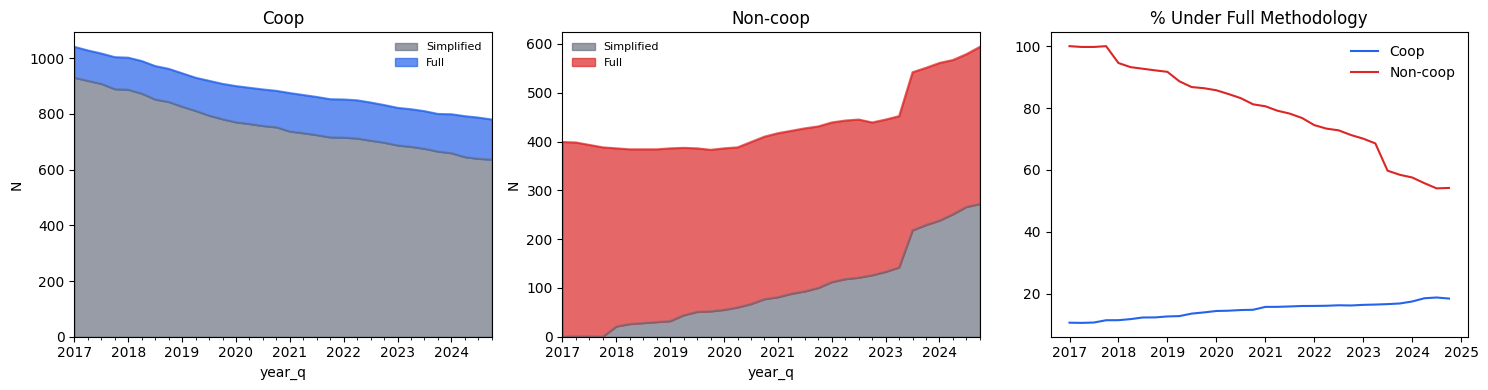
\includegraphics[width=\textwidth]{figures/fig5_regulatory.png}
\caption{Regulatory methodology over time. Panels (a) and (b) show cooperatives and
non-cooperative institutions across the simplified and full methodologies; panel (c)
shows the share under full methodology. The step in the non-cooperative simplified count
from 2023 is the entry of payment-institution-led prudential conglomerates into
prudential reporting under Resolutions BCB 197 to 202 of 2022, in force from July 2023,
which placed them in S4 or, where they opted for the simplified methodology, in S5:
seventy institutions in 2023, all under the simplified methodology, none of which enters
the comparison group used here. Source: authors' calculations from BACEN IF.data.}
\label{fig:regulatory}
\end{figure}

Credit cooperatives are member-owned institutions that take deposits and lend, mostly to
their members, organised under Complementary Law 130/2009 and Resolution 4.434/2015,
which classifies them as \textit{plena}, \textit{cl\'assica} or \textit{de capital e
empr\'estimo} according to the operations they may conduct \citep{lc130, cmn4434}. Resolution
5.051/2022 reorganised the cooperative rules from January 2023, retaining the three-way
classification and revoking the minimum-capital articles of Resolution 4.434; a new
methodology for the minimum paid-in capital and net worth of all authorised institutions
followed in November 2025, after the sample ends \citep{cmn5051, resconj14}. In Brazil cooperatives hold about six percent of
system assets at the end of 2024 and 6.3 percent a year later, and the share has risen
in every year since 2020 \citep{bcb2025panorama, bcb2026panorama}. Much of the sector belongs to
integrated systems in which central cooperatives supply liquidity facilities,
consolidated risk management and a single supervisory interface to their affiliates.
Membership of such a network changes the constraints an individual cooperative faces,
and we test for it below.

\subsection{Theoretical framework}
\label{sec:theory}

Prudential capital regulation exists to internalise the
externalities that a financial institution's failure imposes on depositors, on the
payment system and on the public safety net, and to offset the moral hazard that deposit
guarantees introduce into the institution's own choice of leverage \citep{bcbs2011}. In
the economic theory of banking regulation this rationale is a representation argument: the
supervisor acts on behalf of the small,
dispersed depositors who lack the incentive and the means to monitor a leveraged
intermediary, and the capital requirement substitutes for the discipline those depositors
cannot exert \citep{dewatripont1994}. Its
instruments, a minimum capital definition, minimum ratios and standardised risk
weights, are calibrated to the population the regulator has in mind. That rationale is
not obviously invariant to organisational form. An investor-owned bank funded in
wholesale markets, a member-owned cooperative funded by member deposits, and a cooperative
embedded in an integrated network with a central liquidity facility and a mutual guarantee
differ in the externality their failure generates and in the safety-net arrangement that
stands behind them. The representation channel is the sharpest of these: in a credit
cooperative the depositor is also a member with a residual claim and a governance right,
and, in the integrated systems, a central body supplies consolidated monitoring, so the
representation problem the template is built to solve is partly internalised. The systemic
externality of failure and the moral hazard of a public guarantee are not internalised in
the same way; thinner capital with no offsetting conservatism bears on those rather than on
the monitoring margin. Where those differ, a capital template written for one need not be
neutral when applied to another: it may bind on a margin that does not carry the risk it
was designed to price.

This is the sense in which proportionality is at issue. Brazil's segmentation framework
applies proportionality along a single margin: institution size \citep{cmn4553}. Most
jurisdictions do the same. The Basel Committee's survey of proportionality practices and
the FSI cross-country comparisons find that supervisors scale requirements by size and
complexity, and that tailoring by ownership form is rare \citep{bcbs2019,
castrocarvalho2017, hohl2018}. \citet{coelho2019} review how supervisors in nine
jurisdictions adapt the framework to financial cooperatives specifically, and find
that the adaptation usually concerns capital instruments and network arrangements rather
than the level of the requirement. The regulatory-design literature reads proportionality
more broadly, as the matching of supervisory intensity to the risk and the character of
the regulated firm. Responsive regulation \citep{ayres1992} and its ``really responsive''
development \citep{baldwin2008} treat the attributes of the regulated entity, its
ownership, its incentives and the institutional structure it sits within, as inputs to how
the regime should engage it, escalating where the risk warrants and relaxing where it does
not. On that reading organisational form and network membership are candidate calibration
margins. The reading cuts in both
directions. A cooperative that holds less capital than a comparable bank might, under a
form-sensitive regime, warrant lighter treatment if its risk profile and its network
backstop justify the thinner cushion, or closer scrutiny if they do not. Which of the two
applies is a calibration question, and a descriptive profile of how the two forms differ
under identical rules is the input that question needs; it does not require a causal
estimate of the effect of form.

Why the two forms might differ at all, once the rules are fixed, follows from ownership. A
cooperative cannot raise outside voting equity as needed: its capital is an endowment of retained earnings
accumulated across member generations rather than a claim traded on a market
\citep{fonteyne2007}. Basel III admits member shares of mutuals and cooperatives as
common equity under criteria adapted to their legal form \citep{bcbs2011}, but the shares
remain redeemable claims of members and cannot be placed with outside investors. The
property-rights structure of the member's claim is ill-defined in the
ways \citet{cook1995} sets out: free-rider, horizon, portfolio, control and
influence-cost problems that
weaken members' incentive to build capital beyond what member service requires.
\citet{hansmann1996} frames the same point as a comparison of ownership costs: the
member-owner's residual claim is tied to use of the institution, not to the appreciation
of a tradable investment, so capital accumulation is instrumental to the delivery of
member credit rather than an objective in its own right. This structure predicts a
recognisable configuration: capital that is thinner and less dispersed than in an
investor-owned population that can raise and price equity externally, and a balance sheet
tilted toward member lending.

\subsection{Comparison groups in the cooperative banking literature}

\citet{mckillop2020} survey the field. Three strands matter here. The first concerns
capital, profitability and stability. \citet{hesse2007} find cooperative banks more
stable than commercial banks in a cross-country panel, driven by lower volatility of
returns, which more than offsets lower profitability and lower capitalisation.
\citet{iannotta2007} find that ownership structure predicts risk and performance across
European banks of similar size, and \citet{beck2009} find the same within a single
regulatory regime in Germany. \citet{ayadi2010} document the business-model differences
across European cooperative banks, and \citet{bulbul2013}
show for European savings and cooperative banks that ownership and governance shape
business models across regulatory environments. \citet{fiordelisi2014} follow the stability of cooperative banks through the
financial crisis and \citet{becchetti2016} their lending. \citet{ferri2014} show that ownership form shapes lending behaviour in
the euro area. \citet{cuevas2006} set out the tension between member orientation and
prudential templates written for investor-owned banks, and \citet{fonteyne2007} the
capital problem: a cooperative cannot raise outside voting equity as needed, so its buffer is an
intergenerational endowment of retained earnings.

The second strand concerns proportionality. The policy question is whether rules
calibrated for large, complex, internationally active banks suit small and locally
focused institutions, and whether organisational form belongs in the calibration
\citep{bcbs2019, castrocarvalho2017, coelho2019}.

The third strand is Brazilian. \citet{bressan2011} apply the PEARLS system to Brazilian
credit cooperatives and model their insolvency risk. \citet{carvalho2015} analyse the exit
and failure of Brazilian credit unions. The Central Bank's own studies compare
cooperatives with private banks on credit-market share and on the behaviour of newly
captured clients \citep{bcb2018ee14, bcb2020ee91}, and its annual \textit{Panorama}
tracks the sector \citep{bcb2025panorama}. None of these compares cooperatives with banks
under a common prudential methodology, which is the setting used here.

Something is asked less often. When a paper reports that cooperative banks are less
profitable, or better capitalised, or more conservative than banks, the claim is
relative to a comparison group, and papers often do not say which institutions belong
to it. Regulatory populations are defined by legal or consolidation category, not by
economic function, so they can include institutions that neither lend nor take
deposits. Our data show that this is not a small problem. Of the 483 non-cooperative
institutions under full methodology in Brazil, 196 report a median credit-to-assets
ratio of zero and a median funding ratio of zero.

% entregar um pouco do resultado na introdução para o leitor não ter que esperar até a seção de resultados pra saber.
\subsection{This paper}

We study the population of Brazilian institutions that compute capital, risk-weighted
assets and provisions under the full Basel methodology between 2017 and 2024, comprising 130 singular
credit cooperatives and 144 banks, 7{,}234 institution-quarters, and ask whether
organisational form leaves an imprint on the balance sheet once the rulebook is held
fixed. We compare cooperatives with banks across a ladder of comparison groups defined on
the regulator's own categories, correct two features of the source data that would
otherwise distort the rate variables, and report how far each result depends on the
comparison group, the rate construction and the weighting of the matched estimator.

At comparable size, cooperatives allocate about nineteen percentage points more of assets
to credit than banks, earn some two percentage points more on assets, and run markedly
leaner cost-to-income ratios, with less volatile returns and a higher distance to
insolvency, while holding less regulatory capital. The capital gap is
large at the mean, around two percentage points at the conditional median, and belongs to
the integrated cooperative systems rather than to the form as such. Two differences that
look large against a broad comparison group do not survive the comparison with banks:
cooperatives provision no differently, and their intermediation margin is indistinguishable
from that of banks. A benchmark calibrated on the average full-methodology institution
therefore describes cooperatives poorly, because cooperatives do not populate the
distribution that average is drawn from.

% =============================================================================
\section{Aims}
% =============================================================================

%\subsection{Predictions}
%\label{sec:aims}

The framework generates expectations we take to the data. We state them as directional
predictions where the theory commits to a sign and leave them open where it does not.

We ask, first, whether organisational form leaves a measurable imprint on capital,
profitability, efficiency, stability, credit allocation and funding once the regulatory
environment is held fixed. The ownership account commits to a sign in two places. Because a cooperative
cannot raise or price equity externally and builds capital only as a retained-earnings
endowment, we expect cooperatives to hold less regulatory capital than banks of comparable
size, and to occupy a narrower band of the capital distribution than a population that can
issue equity on demand. Because the member's residual claim is a claim on use rather than
on investment return, we expect the balance sheet to tilt toward member credit, so that
cooperatives allocate a higher share of assets to lending than comparable banks. The
framework does not fix the sign of the profitability and efficiency comparison: a
member-service orientation is consistent both with surplus returned to members through
pricing, which would depress the return on assets, and with the cost discipline of a
focused retail model, which would raise it. We treat that comparison as open. On the
volatility of returns the account gives a direction: a cooperative that prices to members
can absorb shocks through the surplus it would otherwise return, which \citet{hesse2007}
identify as the source of cooperative stability, so we expect lower return volatility and a
greater distance to insolvency at comparable size. For
provisioning and the intermediation margin the framework offers no reason to expect a
difference at all: minimum provisions are fixed by the AA--H rating grid under Resolution
2.682/1999 \citep{cmn2682} rather than by ownership, so a difference on either, if one
appears, is more likely to reflect the composition of the comparison group than the effect
of form.

We ask, second, how much the answer to the first question depends on choices the analyst
makes. We examine three: which institutions form the comparison
group, how cumulative accounting flows are converted into rates, and how a matched
estimator is weighted. Each is a choice most papers report in a sentence, if at all, and
each turns out to determine whether a headline result exists. This is a question about
method, and we do not frame it as a prediction.

% =============================================================================
\section{Methods}
% =============================================================================

\subsection{Data}

We build an institution-level quarterly panel from IF.data, the public statistical
repository of the Central Bank of Brazil. We merge the summary financials, the
segmentation file, the asset composition file and the income statement on institution
code and reporting date. Each source is deduplicated on the institution-quarter key
before merging. The asset composition module carries 1,354 duplicate institution-quarter
rows against three in the other modules, and we collapse them to the most complete
record. An arbitrary choice among duplicates moves the credit and provisioning
variables. The raw panel runs from 2014Q1 to 2024Q4 and contains 61,377
institution-quarters on 1,959 institutions.

\subsection{Classification}

We classify institutions on the Central Bank's consolidation type,
\textit{tipo de consolidado banc\'ario} (\texttt{tcb}). Two values identify the
cooperative sector: \texttt{b3S} is a singular credit cooperative and \texttt{b3C} a
central cooperative or confederation. Consolidation type is a regulatory attribute rather
than a feature of a trade name, so it is stable over time. We assign each institution its
modal \texttt{tcb} over the period, which makes cooperative status time-invariant by
construction.

We exclude central cooperatives. They are wholesale entities that supply liquidity and
risk management to affiliated singulars, they carry high capital for structural reasons,
and pooling them with retail cooperatives mixes the retail profile with the sector's
infrastructure.

Classification by name has a specific failure mode in this setting. A name-based rule
places the cooperative sector's own banks, Banco Cooperativo Sicredi and Banco Sicoob,
both \texttt{b1} commercial banks, in the cooperative group. One institution then appears
on both sides of the comparison and cooperative status is no longer time-invariant.

\subsection{Comparison groups}
\label{sec:peers}

The cooperative side is always the singular retail cooperatives under full methodology.
The comparison side is a choice. We make it a reported parameter and define the
alternatives on the regulator's consolidation type, never on an outcome:

\begin{itemize}
\item all non-cooperatives: every full-methodology institution outside the \texttt{b3}
family, 483 institutions;
\item bank-like: \texttt{b1}, \texttt{b2} and \texttt{b4} (development banks);
\item banks: \texttt{b1} commercial and multiple banks with a commercial portfolio and
\texttt{b2} multiple and investment banks, 144 institutions;
\item commercial: \texttt{b1} only, 105 institutions.
\end{itemize}

Banks is the primary group. Of the 483 institutions in the broad group, 335 are non-banking institutions.
Nearly two hundred of these hold no credit and take no deposits, which makes the credit
and funding differentials mechanical. For the smallest of them the methodology flag is
itself doubtful: forty non-bank credit institutions with median assets near two million
reais are recorded as not using the simplified computation while remaining in segment 5,
which at that size more plausibly records that the simplified computation does not apply
than that the full apparatus does. We report the
broad group throughout, since the divergence between the two is one of our results.

\subsection{Outcomes and two measurement corrections}
\label{sec:measurement}

We study eight quarterly outcomes: the Basel capital ratio and leverage (liabilities over
assets); return on assets and the intermediation margin; the cost-to-income ratio; the
credit portfolio over assets and a provisioning ratio; and funds raised over assets. Two
features of IF.data affect how these are built.

We add two stability outcomes measured at the institution level over its
full-methodology quarters: the standard deviation of annualised quarterly return on
assets, and the z-score, mean return on assets plus mean equity-to-assets over the
standard deviation of return on assets, the distance-to-insolvency measure of
\citet{hesse2007}. Both require at least eight quarters. The rule leaves 105
cooperatives and 137 banks; the 25 cooperatives it drops are late entrants to the full
methodology. Because the unit is the institution, these two outcomes are estimated on one
row per institution with mean log assets as the size control, no quarter effects, HC3
standard errors and a wild bootstrap over institutions. Their rows in the tables are
marked accordingly.

Income flows accumulate within the semester. Financial institutions in Brazil are
required to draw up general balance sheets on 30 June and 31 December (Lei 4.595/1964,
art.~31), and IF.data income statement fields follow this convention: they run from
January to June, reset, and run again from July to December. The median ratio of the fourth-quarter to the
first-quarter value is 2.27 for every income field and 1.09 to 1.11 for balance sheet
stocks. Median second-to-first and fourth-to-third quarter ratios are 2.11 and 2.07.
Read as quarterly flows, these fields make return on assets a one-quarter return in the
first and third quarters and a two-quarter return in the second and fourth, so the ratio
averages inconsistent horizons. We de-cumulate within each semester and annualise.
The correction scales the flow-based coefficients by about 2.7 and leaves every
stock-based coefficient unchanged.

The intermediation result is net of loan loss provisions. The IF.data expense subtotal
$(b)$ contains line $(b5)$, \textit{Resultado de Provis\~ao para Cr\'editos de Dif\'icil
Liquida\c{c}\~ao}, so $(c) = (a) + (b)$ is not a net interest margin. Built that way, the
margin variable partly reproduces the provisioning result under another name. The overlap
is small in the unconditional specification and about a quarter of the coefficient in the
trimmed one. We compute the margin gross of $(b5)$, and the cost-to-income denominator
likewise.

We use the term provisioning ratio rather than a non-performing-loan ratio. The variable
is the stock of provisions constituted under Resolution 2.682/1999 over gross credit.
Under that regime the minimum provision is a step function of the AA--H risk rating
assigned to each operation, so the ratio reflects how the institution classifies its
book rather than realised delinquency.

\begin{table}[htbp]
\centering
\small
\caption{Outcome definitions}
\label{tab:defs}
\begin{threeparttable}
\begin{tabular}{lp{10.2cm}}
\toprule
Outcome & Construction \\
\midrule
Basel capital ratio & \textit{Índice de Basileia} as reported by BACEN: regulatory
capital over risk-weighted assets, in percentage points \\
Leverage & Total liabilities / total assets \\
Return on assets & $4 \times$ (quarterly net income) / total assets, where quarterly net
income is line (j) de-cumulated within the semester \\
Intermediation margin & $4 \times [(c) - (b5)]\,/$ total assets, de-cumulated within the
semester: the intermediation result gross of the loan-loss line \\
Cost-to-income & $[|(d3)| + |(d4)|] \,/\, [(c) - (b5) + |(d2)|]$, all de-cumulated within
the semester: personnel and administrative expense over operating income gross of
provisions \\
Credit portfolio / assets & Credit portfolio / total assets \\
Provisioning ratio & Stock of credit provisions constituted under Res.~2.682/1999 /
gross credit \\
Funding ratio & \textit{Captações} (funds raised) / total assets \\
\midrule
Return volatility & Standard deviation of annualised quarterly return on assets across
the institution's full-methodology quarters (institution level, at least eight
quarters) \\
Z-score & [mean return on assets $+$ mean $(1 - \text{leverage})$] / standard deviation
of return on assets (institution level, at least eight quarters) \\
\bottomrule
\end{tabular}
\begin{tablenotes}[flushleft]\footnotesize
\item IF.data income statement lines: (c) intermediation result, (b5) loan-loss
provision result, (d2) fee income, (d3) personnel expense, (d4) administrative expense,
(j) net income. A ratio of two flows over the same window is invariant to annualisation;
a ratio of a flow to a stock is not. This is why the semester correction moves return on
assets and the margin but leaves the four stock-based outcomes numerically unchanged.
\end{tablenotes}
\end{threeparttable}
\end{table}

\subsection{Specifications}

For each outcome $y$ we estimate the coefficient on a cooperative indicator under four
specifications. The first is the unconditional difference in means. The second adds log
total assets and quarter fixed effects. The third is coarsened exact matching
\citep{iacus2012} with the same controls. The fourth restricts the sample to the region
of common support in log assets and applies the same controls.

Cooperative status does not vary within an institution, so it is collinear with any
institution fixed effect. The estimates are conditional correlations. We do not present
them as causal effects of organisational form.

\subsection{Matching}
\label{sec:cem}

The coarsened-exact-matching estimand weights control
units so that the treated-to-control ratio is equal within every stratum
\citep{iacus2012}; OLS on the matched sample does not recover it. Unweighted, strata are
implicitly weighted by their control counts. In
our data a stratum holding two cooperatives and ninety-three banks would count some two
hundred and fifty times more heavily, relative to its share of cooperatives, than a
stratum holding thirty-eight cooperatives and seven banks. We report the weighted
estimand and the unweighted matched-sample regression together.

We coarsen on size quintile and control for region. We do not exact-match on
macro-region. Cooperatives concentrate in the South and banks in the Southeast, so
region-exact strata leave an effective control sample of about eighteen institutions by
the Kish measure, with weights ranging from 0.07 to 10.96. Under size-quintile coarsening
the weights run from 0.41 to 1.80 and the effective control sample is about
seventy-six. There is also a substantive reason. Brazilian cooperatives are concentrated
where they are for reasons internal to member-based finance, so region is plausibly a
mediator of cooperative form rather than a confounder of it, and conditioning on it
removes part of the effect. We report region-exact estimates as a within-market bound.

\subsection{Inference}
\label{sec:inference}

Standard errors are clustered by institution. Institutions are observed for up to
thirty-two quarters, their observations are serially correlated, and cooperative status
is assigned at the institution level \citep{cameron2015, abadie2023}. We also compute
heteroskedasticity-robust errors \citep{mackinnon1985}, which are uniformly tighter, so
the clustered errors are the conservative choice.

We compute a restricted wild cluster bootstrap with Rademacher weights and 1{,}999
replications for every coefficient \citep{cameron2008}. Cluster-robust inference is
unreliable when the number of treated clusters is small \citep{mackinnon2017}, which is
the case in the system-by-system estimates. In simulations on our design, with six
treated clusters drawn at random and two hundred draws, the cluster-robust test rejects a
true null 16 percent of the time at a nominal 5 percent level and 10 percent of the time
at a nominal 1 percent level. The wild bootstrap rejects 10 and 0.5 percent respectively:
it is correctly sized at the 1 percent level and closer to size at 5 percent. With a true
effect the median bootstrap $p$-value is 0.03. With more than a hundred treated clusters
the two tests agree. We report treated cluster counts beside every system-level estimate.
With five treated clusters there are $2^5$ treated sign patterns, so the smallest
attainable bootstrap $p$-value is of the order of 0.03; the figure is approximate rather
than a bound, since the control clusters' signs also move the statistic.

\subsection{Means and medians}

Several outcomes are right-skewed. The Basel ratio has a skewness above four in the
analysis sample and the cost-to-income ratio above four, because a minority of banks
carry very high capital ratios or very low operating income. We report the conditional
median alongside the conditional mean for every outcome.

% =============================================================================
\section{Results}
\label{sec:results}
% =============================================================================

The analysis sample contains 130 singular cooperatives and 144 banks, 7,234
institution-quarters, from 2017Q1 to 2024Q4. Ninety percent of cooperative observations but only forty-eight percent of bank
observations fall inside the common support region of log assets, which runs from 11.39 to
15.68 (Figure~\ref{fig:overlap}). The asymmetry is itself informative: cooperatives occupy
a narrow band of a size distribution across which banks are spread, so half the bank
population has no cooperative counterpart at any size.

The comparison runs almost entirely within one segment. Ninety-nine percent of
cooperative observations are in S4; among banks, 62 percent are in S4 and 30 percent in
S3. Segments 1 and 2 account for 362 of 4{,}176 bank observations and contain no
cooperative at all.

Two features of the sample govern how the estimates read. Cooperatives are smaller than
the banks they are compared with: the standardised difference in log assets is $-0.72$
before matching, $-0.09$ after matching and $0.01$ after trimming. Comparisons that do
not hold size constant therefore compare cooperatives with larger institutions.
Cooperatives also occupy a narrower band of the size distribution than banks, and, as
the capital results show, a narrower band of the capital distribution.

\begin{figure}[htbp]
\centering
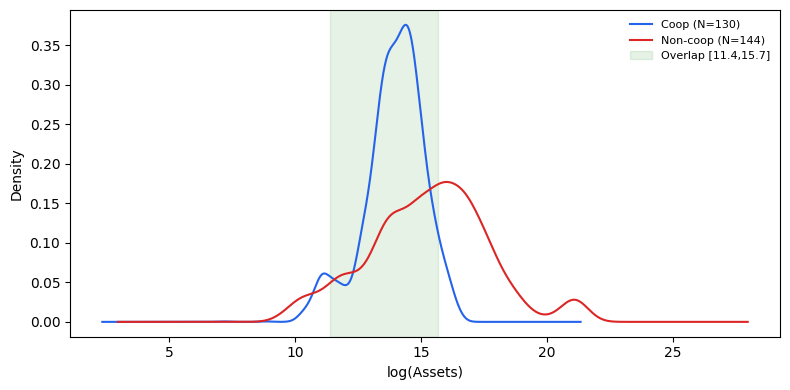
\includegraphics[width=0.78\textwidth]{figures/fig8_overlap.png}
\caption{Common support in log total assets, cooperatives and banks. The shaded region
marks the overlap. Source: authors' calculations from BACEN IF.data.}
\label{fig:overlap}
\end{figure}

Table~\ref{tab:desc} reports unconditional means and medians.

\begin{table}[htbp]
\centering
\begin{threeparttable}
\caption{Unconditional means and medians, analysis sample}
\label{tab:desc}
\begin{tabular}{lrrrrrr}
\toprule
 & \multicolumn{2}{c}{Cooperatives} & \multicolumn{2}{c}{Banks} & \multicolumn{2}{c}{Observations} \\
\cmidrule(lr){2-3}\cmidrule(lr){4-5}\cmidrule(lr){6-7}
Outcome & Mean & Median & Mean & Median & Coop. & Banks \\
\midrule
Basel capital ratio (pp) & 22.77 & 20.46 & 30.96 & 18.41 & 3,048 & 4,170 \\
Leverage & 0.8337 & 0.8493 & 0.7777 & 0.8644 & 3,048 & 4,184 \\
Return on assets (ann.) & 0.0288 & 0.0284 & 0.0108 & 0.0116 & 3,048 & 4,181 \\
Cost-to-income ratio & 0.5536 & 0.5516 & 1.1561 & 0.6455 & 3,048 & 3,853 \\
Credit portfolio / assets & 0.5673 & 0.5899 & 0.4020 & 0.3956 & 3,048 & 4,184 \\
Provisioning ratio & 0.0546 & 0.0503 & 0.0527 & 0.0322 & 2,945 & 3,520 \\
Intermediation margin (ann.) & 0.0839 & 0.0809 & 0.0842 & 0.0516 & 3,048 & 4,181 \\
Funding ratio & 0.6156 & 0.6114 & 0.5694 & 0.6752 & 3,048 & 4,184 \\
\bottomrule
\end{tabular}
\begin{tablenotes}[flushleft]\footnotesize
\item Unconditional. The median cooperative Basel ratio exceeds the median bank ratio while the size-adjusted differential in Table 3 is negative: cooperatives are smaller than the banks in this population and capital ratios fall with size.
\end{tablenotes}

\end{threeparttable}
\end{table}

\subsection{The cooperative differential}

Table~\ref{tab:main} reports the cooperative coefficient under the four specifications,
with the conditional median counterpart of the second column and the retention ratio
$\rho = |\beta_{\text{trim}}| / |\beta_{\text{raw}}|$.

\begin{table}[htbp]
\centering
\begin{threeparttable}
\caption{Cooperative differential against banks, four specifications}
\label{tab:main}
\footnotesize
\setlength{\tabcolsep}{4pt}
\begin{tabular}{lrrrrrrl}
\toprule
Outcome & (1) Raw & (2) Controls & (3) CEM & (4) Trim & Median (2) & $\rho$ & Tier \\
\midrule
Basel capital ratio (pp) & -8.19$^{***}$ & -15.77$^{***}$ & -17.50$^{***}$ & -14.21$^{***}$ & -2.18 & 1.73 & robust \\
Leverage & 0.0561$^{**}$ & 0.1220$^{***}$ & 0.1046$^{***}$ & 0.0813$^{***}$ & 0.0283 & 1.45 & robust \\
Return on assets (ann.) & 0.0181$^{***}$ & 0.0215$^{***}$ & 0.0179$^{***}$ & 0.0159$^{***}$ & 0.0171 & 0.88 & robust \\
Cost-to-income ratio & -0.6025$^{***}$ & -0.7923$^{***}$ & -0.8385$^{***}$ & -0.7522$^{***}$ & -0.1796 & 1.25 & robust \\
Credit portfolio / assets & 0.1654$^{***}$ & 0.1881$^{***}$ & 0.1701$^{***}$ & 0.1780$^{***}$ & 0.2448 & 1.08 & robust \\
Provisioning ratio & 0.0020 & -0.0012 & 0.0010 & 0.0009 & 0.0236 &  & null \\
Intermediation margin (ann.) & -0.0003 & -0.0190 & -0.0107 & -0.0171 & 0.0203 &  & null \\
Funding ratio & 0.0461 & 0.0887$^{**}$ & 0.0536 & 0.0330 & -0.0247 &  & null \\
\midrule
Return on assets volatility & -0.0110$^{***}$ & -0.0189$^{***}$ & -0.0175$^{***}$ & -0.0170$^{***}$ & -0.0133 & 1.55 & robust \\
Z-score & 4.20$^{***}$ & 6.32$^{***}$ & 6.14$^{***}$ & 6.20$^{***}$ & 7.58 & 1.48 & robust \\
\bottomrule
\end{tabular}
\begin{tablenotes}[flushleft]\footnotesize
\item Coefficient on the cooperative indicator; standard errors clustered by institution. Every starred cell was additionally checked with a restricted wild cluster bootstrap (1,999 replications), which agrees with the clustered test throughout. 'Median (2)' is the conditional-median counterpart of column (2). rho = |b\_trim|/|b\_raw|, reported only when all four columns are significant; rho above one means the differential grows as the design tightens. The final two rows are institution-level stability outcomes (return-on-assets volatility and the z-score, one value per institution over its full-methodology quarters); they are estimated on an institution-level cross-section with HC3 errors and a wild bootstrap over institutions, and their stars are HC3.
\end{tablenotes}

\end{threeparttable}
\end{table}

Five of the eight quarterly outcomes hold their sign and significance across all four
specifications, across
coarsening schemes, and across winsorisation rules including no winsorisation
(Figure~\ref{fig:stability}). None of
them attenuates. The retention ratio is 1.73 for the capital ratio, 1.45 for leverage,
1.25 for cost-to-income, 1.08 for credit intensity and 0.88 for return on assets.
Controlling for size, matching, and trimming to common support make these differentials
larger, which is not what a size-composition artefact does.

Cooperatives allocate more of the balance sheet to credit. The differential is 0.188 in
the controlled specification and moves little across the four columns. It is the most
stable result in the study. It changes by less than one percentage point across
winsorisation rules, from 0.187 with no winsorisation to 0.193 under tight clipping, and
it is larger at the conditional median, 0.245, than at the mean.

Cooperatives earn more on assets. The annualised differential is 2.1 percentage points
under controls and 1.7 at the conditional median. In banking this is a large gap. It
coexists with an intermediation margin that is statistically indistinguishable from that
of banks, so the return comes from volume and cost rather than from wider spreads.

Cooperatives run leaner. The cost-to-income differential is negative and significant
everywhere. Its magnitude is sensitive to the tail, ranging from $-0.46$ under tight
winsorisation to $-1.40$ with none, with a conditional median of $-0.18$.

The capital result is the one that most needs care, because the conditional mean does not
describe the typical institution. Unconditionally the median cooperative is better capitalised
than the median bank, 20.5 percent against 18.4, and Figure~\ref{fig:series} shows the
cooperative median above the bank median for most of the window. The size-controlled mean
differential is nonetheless large and negative: $-8.2$ percentage points unconditionally,
$-15.8$ with size controls, $-17.5$ under matching and $-14.2$ on common support.

Table~\ref{tab:quant} and Figure~\ref{fig:quantiles} reconcile the two. The cooperative
coefficient is positive at the bottom of the conditional capital distribution and negative at
the top, crossing zero near the fortieth percentile: $+2.8$ percentage points at the tenth,
$+1.3$ at the thirtieth, $-2.2$ at the median, $-19.3$ at the eightieth and $-34.4$ at the
ninetieth. Averaged over the twentieth to eightieth percentiles the differential is $-5.1$,
about a third of the conditional mean. The unconditional deciles say the same. Cooperatives
are above banks at every decile up to the sixtieth and below thereafter, and while 53 percent
of cooperatives hold a Basel ratio above 20 percent against 44 percent of banks, 14 percent of
banks exceed 50 percent against 1 percent of cooperatives.

The mean gap describes the bank upper tail. What separates the two groups at equal size is
dispersion (Table~\ref{tab:disp}). The standard
deviation of the capital ratio, residualised on size and quarter, is 9.2 for cooperatives and
29.7 for banks; the interquartile range is 8.4 against 18.3.

\begin{table}[htbp]
\centering
\begin{threeparttable}
\caption{Cooperative coefficient across the conditional distribution}
\label{tab:quant}
\small
\setlength{\tabcolsep}{5pt}
\begin{tabular}{lrrrrrr}
\toprule
Outcome & $q_{10}$ & $q_{25}$ & $q_{50}$ & $q_{75}$ & $q_{90}$ & Mean \\
\midrule
Basel Capital Ratio (\%) & 2.81 & 1.61 & -2.18 & -14.23 & -34.37 & -15.77 \\
Leverage (liabilities/assets) & 0.2943 & 0.1168 & 0.0283 & -0.0093 & -0.0228 & 0.1220 \\
Return on Assets & 0.0440 & 0.0255 & 0.0171 & 0.0098 & -0.0057 & 0.0215 \\
Cost-to-Income Ratio & 0.1096 & 0.0062 & -0.1796 & -0.6469 & -1.7561 & -0.7923 \\
Credit Portfolio / Assets & 0.3827 & 0.4242 & 0.2448 & -0.0185 & -0.1702 & 0.1881 \\
Provisioning (provisions/gross credit) & 0.0301 & 0.0299 & 0.0236 & 0.0008 & -0.0539 & -0.0012 \\
\bottomrule
\end{tabular}
\begin{tablenotes}[flushleft]\footnotesize
\item Cooperative coefficient from quantile regressions of each outcome on the cooperative indicator, log assets and quarter fixed effects, at five quantiles of the conditional distribution, with the OLS conditional mean for comparison. Where the coefficient changes sign across quantiles, the mean describes neither tail.
\end{tablenotes}

\end{threeparttable}
\end{table}

\begin{figure}[htbp]
\centering
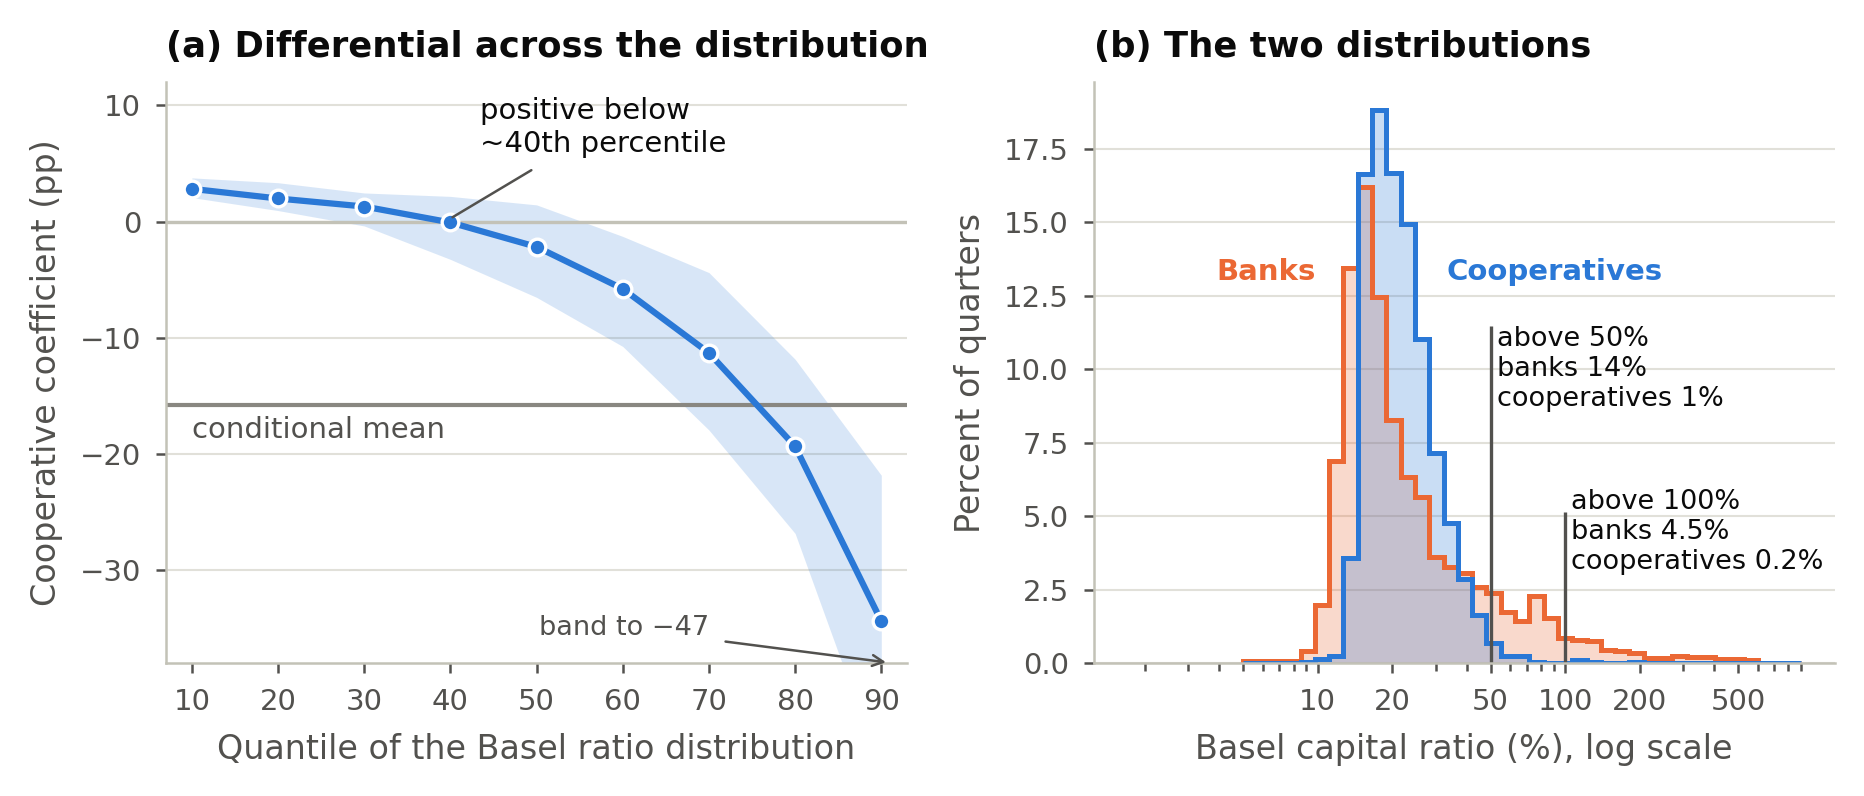
\includegraphics[width=\textwidth]{figures/fig12_capital_quantiles.png}
\caption{The capital differential across the distribution. Panel (a) plots the cooperative
coefficient from quantile regressions of the Basel ratio on the cooperative indicator, log
assets and quarter fixed effects, against the conditional mean. Panel (b) plots the two
unconditional distributions. Source: authors' calculations from BACEN IF.data.}
\label{fig:quantiles}
\end{figure}

The pattern extends to the other outcomes and governs how each should be read. Averaged over
the twentieth to eightieth percentiles the differential is 116 percent of the conditional mean
for credit intensity and 80 percent for return on assets, so for those two the mean describes
the typical institution. For leverage it is 38 percent and for cost-to-income 35 percent, and
both change sign inside the distribution: banks are leaner than cooperatives at the efficient
end and much less lean at the inefficient end. Cooperatives are the more homogeneous group on
every outcome at equal size, with residual standard deviations between a tenth and a half of
the bank figure.

\begin{table}[htbp]
\centering
\begin{threeparttable}
\caption{Dispersion at equal size: residual standard deviation and interquartile range}
\label{tab:disp}
\small
\setlength{\tabcolsep}{5pt}
\begin{tabular}{lrrrrr}
\toprule
 & \multicolumn{2}{c}{Residual s.d.} & & \multicolumn{2}{c}{Residual IQR} \\
\cmidrule(lr){2-3}\cmidrule(lr){5-6}
Outcome & Coop. & Banks & Ratio & Coop. & Banks \\
\midrule
Basel Capital Ratio (\%) & 9.2379 & 29.7383 & 0.31 & 8.3718 & 18.3313 \\
Leverage (liabilities/assets) & 0.0759 & 0.1788 & 0.42 & 0.0793 & 0.1429 \\
Return on Assets & 0.0180 & 0.0420 & 0.43 & 0.0174 & 0.0225 \\
Return on Assets, pre-tax & 0.0185 & 0.0553 & 0.33 & 0.0179 & 0.0340 \\
Cost-to-Income Ratio & 0.1491 & 1.4751 & 0.10 & 0.1859 & 0.7334 \\
Credit Portfolio / Assets & 0.1208 & 0.3088 & 0.39 & 0.1486 & 0.5459 \\
Provisioning (provisions/gross credit) & 0.0243 & 0.0701 & 0.35 & 0.0213 & 0.0507 \\
Z-score & 7.4423 & 9.3498 & 0.80 & 8.5542 & 11.2177 \\
\bottomrule
\end{tabular}
\begin{tablenotes}[flushleft]\footnotesize
\item Residuals from a regression of each outcome on log assets and quarter fixed effects. Ratio: cooperative over bank residual standard deviation; below one, cooperatives are the tighter group. The z-score is institution-level, residualised on mean log assets. Over the seven outcomes jointly, the generalised variance ratio is 0.08.
\end{tablenotes}

\end{threeparttable}
\end{table}

Leverage moves with capital, as expected. Cooperatives are more leveraged at comparable
size by 12 percentage points, with the same caveat: banks are slightly more leveraged at
the unconditional median. The correlation between the Basel ratio and leverage among
cooperatives is $-0.84$, so we treat the two as one result.

Cooperatives are more stable. At comparable size the standard deviation of return on
assets is 1.9 percentage points lower and the z-score 6.3 points higher, with a
conditional median of 7.6. Both hold in all four designs and, like the five quarterly
results, grow as the design tightens. The bootstrap $p$-value is at its floor in every
starred cell. The z-score is also less dispersed among cooperatives, with a residual
standard deviation of 7.4 against 9.4 (Table~\ref{tab:disp}). Read with the return on
assets result, the stability finding places cooperatives on the favourable side of the
return-risk trade-off: higher returns and less volatile ones, on the same intermediation
margin.

\begin{figure}[htbp]
\centering
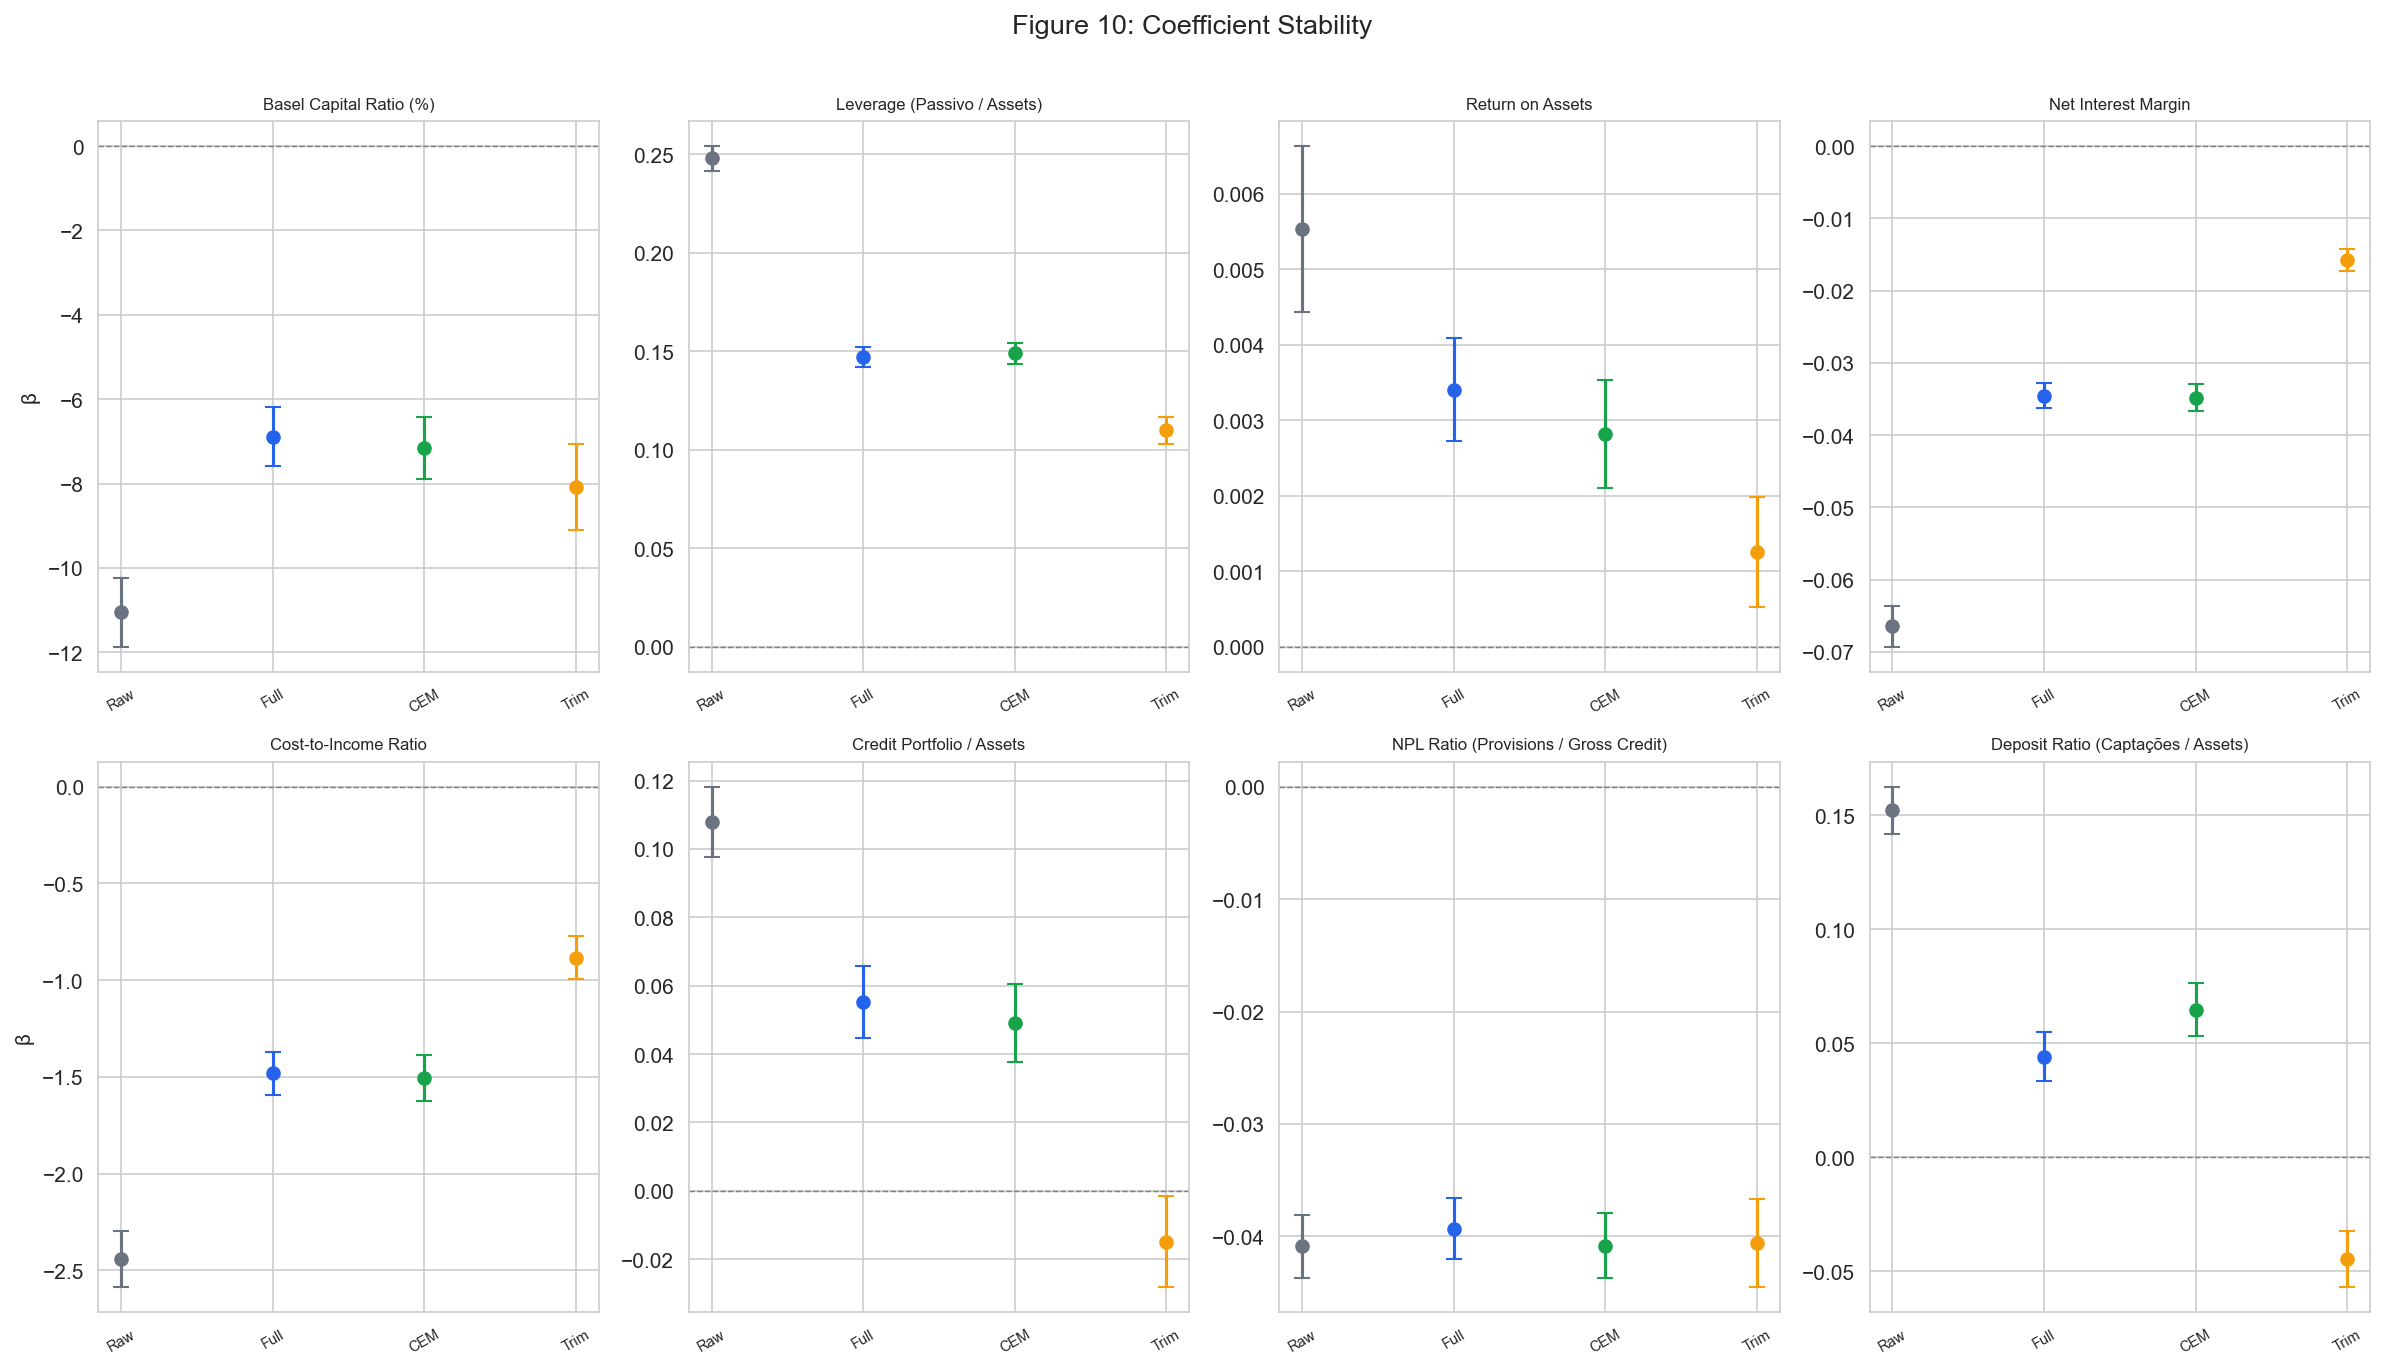
\includegraphics[width=\textwidth]{figures/fig10_stability.png}
\caption{Cooperative coefficient across the four specifications, with confidence
intervals. Source: authors' calculations from BACEN IF.data.}
\label{fig:stability}
\end{figure}

\subsection{What the comparison group determines}

Table~\ref{tab:ladder} re-estimates every outcome against the broad group, against banks,
and against banks matched within macro-region.

\begin{table}[htbp]
\centering
\begin{threeparttable}
\caption{Every outcome across the comparison-group ladder}
\label{tab:ladder}
\small
\setlength{\tabcolsep}{4pt}
\begin{tabular}{lrrr}
\toprule
Outcome & All non-cooperatives & Banks & Banks, within region \\
\midrule
Basel capital ratio (pp) & -8.27$^{***}$ & -15.77$^{***}$ & -7.02$^{*}$ \\
Leverage & 0.1280$^{***}$ & 0.1220$^{***}$ & 0.1052$^{***}$ \\
Return on assets (ann.) & 0.0171$^{***}$ & 0.0215$^{***}$ & 0.0131$^{*}$ \\
Cost-to-income ratio & -1.8277$^{***}$ & -0.7923$^{***}$ & -0.6966$^{*}$ \\
Credit portfolio / assets & 0.2030$^{***}$ & 0.1881$^{***}$ & -0.0254 \\
Provisioning ratio & -0.0330$^{***}$ & -0.0012 & 0.0010 \\
Intermediation margin (ann.) & -0.0910$^{***}$ & -0.0190 & -0.0201 \\
Funding ratio & 0.1768$^{***}$ & 0.0887$^{**}$ & 0.0548 \\
\midrule
Return on assets volatility & -0.0624$^{***}$ & -0.0189$^{***}$ & -0.0170$^{***}$ \\
Z-score & 7.79$^{***}$ & 6.32$^{***}$ & 5.05 \\
\midrule
Comparison institutions & 483 & 144 & 144 \\
\bottomrule
\end{tabular}
\begin{tablenotes}[flushleft]\footnotesize
\item Columns 1 and 2 are the controlled specification and differ only in the comparison group; column 3 additionally exact-matches on macro-region. The broad group includes 196 institutions reporting zero credit and zero deposits. Bank-like (b1+b2+b4) and commercial-only (b1) variants run through the same parameter and are not shown.
\end{tablenotes}

\end{threeparttable}
\end{table}

Two results reported against the broad group do not survive.

Against all non-cooperatives, cooperatives appear to provision 3.3 percentage points
less, significant at one percent in all four specifications with no attenuation. Against
banks the coefficient is $-0.001$ with a $p$-value of 0.86 (0.87 under the bootstrap).
Mean provisioning is 0.055
for cooperatives and 0.053 for banks. The gap in the broad comparison comes from the
non-banking institutions, among which nearly two hundred report no credit and fewer than
five percent report provisions. At the
conditional median the sign reverses, cooperatives provision 2.4 percentage points more,
and under tight winsorisation the mean coefficient is positive and significant at one
percent. We conclude that cooperatives do not provision less than comparable banks. The quantile
estimates support the stronger statement that through most of the distribution they provision
more: the coefficient runs between $+0.024$ and $+0.031$ from the tenth to the fiftieth
percentile and turns negative only in the upper tail, so the zero mean is itself a tail
artefact. Since minimum provisions under Resolution 2.682/1999 are a step function of the
AA--H rating of each operation, this is a statement about how the two groups classify their
credit books.

The intermediation margin behaves the same way. Against the broad group the differential
is $-0.091$ and highly significant. Against banks it is $-0.019$ with a $p$-value of
0.15 (0.16 under the bootstrap), and its sign is not stable across tail treatments. Part of the broad-group result
was the provisioning channel entering through line $(b5)$.

The funding ratio is significant at five percent in one of the four specifications and
marginal in two others, reverses sign at the
conditional median, and falls to insignificance on the common-coverage sample. We do not
report it as a finding. Commercial banks are more deposit-funded than cooperatives at the
unconditional median, 0.675 against 0.611.

\subsection{Credit intensity within and across regional markets}

Matched on size alone, cooperatives allocate 17 to 19 percentage points more of assets to
credit than comparable banks, significant at one percent in every specification. Matched
additionally on macro-region, the differential falls to between $-0.03$ and $+0.07$ and is
not distinguishable from zero under any coarsening scheme.

Cooperatives lend more than the national
bank population but not more than banks operating in the same regional markets. Whether
region is the right thing to condition on depends on whether it is treated as a nuisance
or as part of what cooperative form is. Brazilian cooperatives concentrate in particular
regions for reasons internal to member-based finance, so we take the size-only estimate as
the parameter of interest and the region-matched estimate as a within-market bound.

The z-score follows the same pattern. Its differential is 6.3 against banks nationally
and 5.1, not distinguishable from zero, against banks within macro-region. Return
volatility survives the within-region comparison, so the part of the stability result that
the regional composition does not explain is the volatility of returns.

\subsection{Heterogeneity across cooperative systems: an exploratory split}

Table~\ref{tab:systems} splits the cooperative side by integrated system.

\begin{table}[htbp]
\centering
\begin{threeparttable}
\caption{Cooperative differential by system, controlled specification}
\label{tab:systems}
\begin{tabular}{lrrrrrr}
\toprule
System & Inst. & Treated & Basel (pp) & Leverage & ROA & Provisioning \\
\midrule
Sicredi & 106 & 106 & -17.35$^{***}$ & 0.1341$^{***}$ & 0.0219$^{***}$ & -0.0008 \\
Sicoob & 17 & 17 & -10.98$^{*}$ & 0.0847$^{*}$ & 0.0164$^{*}$ & -0.0007 \\
Independent & 6 & 5 & 6.90 & -0.0313 & 0.0287$^{*}$ & -0.0165 \\
Cresol & 1 & -- & \multicolumn{4}{c}{fewer than five institutions, not estimated} \\
\bottomrule
\end{tabular}
\begin{tablenotes}[flushleft]\footnotesize
\item Each system estimated against the same bank comparison group under the controlled specification. Stars are from a restricted wild cluster bootstrap (Rademacher weights): * p<0.05, ** p<0.01, *** p<0.001. 'Inst.' is the number of cooperatives; 'Treated' is the number of treated clusters that carry a usable observation, which governs reliability. The independent group lists six cooperatives but one contributes no usable observation, so five treated clusters enter every estimate; with five treated clusters the smallest attainable bootstrap p-value is about 0.03. Sicoob's capital coefficient has a bootstrap p-value of 0.019. The independent return-on-assets coefficient carries an asymptotic p-value below 0.001 but a bootstrap p-value of 0.033, the expected gap when only five clusters are treated.
\end{tablenotes}

\end{threeparttable}
\end{table}

The capital pattern belongs to the integrated networks. Sicredi's 106
cooperatives\footnote{The \textit{Panorama} reports 103 Sicredi singulars at December
2024 \citep{bcb2025panorama}. The panel counts every cooperative observed under the full
methodology in any quarter from 2017 to 2024, and the network has consolidated over the
window.} hold
17.3 percentage points less regulatory capital than comparable banks and Sicoob's
seventeen hold 11.0 points less. Both survive the bootstrap, with $p$-values below 0.001
and of 0.019. Six cooperatives are assigned to the independent group, but one contributes no
usable observation, so the independent estimates rest on five treated clusters, three of
which supply nearly all the quarters. They carry a positive point estimate on capital
that cannot be separated from noise, and we present it as
descriptive. Their return on assets shows why the bootstrap matters here: the clustered
$p$-value is below $10^{-8}$ and the bootstrap $p$-value is 0.033, close to the floor
that five treated clusters allow (Section~\ref{sec:inference}).

One hypothesis the split suggests, and cannot test, is a network backstop: cooperatives
with access to centralised liquidity and consolidated risk management may operate on a
thinner individual cushion because the system stands behind them, while an independent
cooperative must self-insure. We record this as a hypothesis generated by the data rather
than an explanation established by it. Nothing here distinguishes it from the other
respects in which the systems differ, including the size, geography and business mix of
their affiliates. What the split does show is that the pooled capital differential
belongs to the system-affiliated segment rather than to the cooperative form as such.
Provisioning is insignificant in every system.

\subsection{Selection into the analysis sample}
\label{sec:selection}

The full-methodology restriction equalises the regulatory environment and it also selects
the sample. The cooperatives we observe are the largest in the country, about a tenth of all
cooperatives ever recorded in the panel. The population described throughout is the set of
Brazilian credit cooperatives subject to the full prudential methodology. Fifty-one
singular cooperatives are observed under the
simplified methodology before they move to the full methodology during the window, so
their behaviour before adoption is observed under the simplified
regime.\footnote{A further five cooperatives in the analysis sample carry
simplified-methodology quarters only after their first full-methodology quarter. They are
the reverters discussed in Section~\ref{sec:robustness} and are excluded from the
pre-adoption comparison; including them and their post-reversion quarters leaves every
sign below unchanged.}

We compare those future adopters with cooperatives that never adopt, while both are under
simplified rules and using only quarters before adoption, conditioning on size and
quarter. There is no detectable difference in leverage ($p=0.29$). Future adopters were
less credit-intensive ($-0.068$, $p=0.003$) and marginally less profitable ($p=0.10$),
and both differences run against our findings: we report that cooperatives out-lend and
out-earn banks. They were also somewhat leaner, by 0.03 on cost-to-income at $p=0.08$,
which runs with the cost-to-income finding. Selection into the sample therefore biases
the credit and profitability estimates toward zero and, if anything, the efficiency
estimate marginally away from it.

\subsection{Robustness}
\label{sec:robustness}

Table~\ref{tab:meanmed} reports the conditional mean and conditional median for every
outcome. The three surviving results with agreeing signs and comparable magnitudes are
credit intensity, return on assets and, in sign, the capital and leverage pair. Where the
median is far smaller than the mean, we report the range rather than the mean alone.

\begin{table}[htbp]
\centering
\begin{threeparttable}
\caption{Conditional mean and conditional median}
\label{tab:meanmed}
\small
\setlength{\tabcolsep}{4pt}
\begin{tabular}{lrrrrc}
\toprule
Outcome & Conditional mean & Conditional median & Ratio & Skewness & Same sign \\
\midrule
Basel capital ratio (pp) & -15.77$^{***}$ & -2.18 & 0.14 & 4.06 & yes \\
Leverage & 0.1220$^{***}$ & 0.0283 & 0.23 & -2.70 & yes \\
Return on assets (ann.) & 0.0215$^{***}$ & 0.0171 & 0.80 & -1.68 & yes \\
Cost-to-income ratio & -0.7923$^{***}$ & -0.1796 & 0.23 & 4.46 & yes \\
Credit portfolio / assets & 0.1881$^{***}$ & 0.2448 & 1.30 & -0.34 & yes \\
Provisioning ratio & -0.0012 & 0.0236 & -19.49 & 3.36 & \textbf{no} \\
Intermediation margin (ann.) & -0.0190 & 0.0203 & -1.07 & 3.86 & \textbf{no} \\
Funding ratio & 0.0887$^{**}$ & -0.0247 & -0.28 & -1.07 & \textbf{no} \\
\bottomrule
\end{tabular}
\begin{tablenotes}[flushleft]\footnotesize
\item Controlled specification, cooperatives against banks. A ratio well below one means the mean differential is produced by the tail of the outcome distribution rather than by the typical institution; a sign disagreement means the mean result does not describe the centre of the distribution.
\end{tablenotes}

\end{threeparttable}
\end{table}

\begin{table}[htbp]
\centering
\begin{threeparttable}
\caption{Excluding the segments where prudential requirements differ}
\label{tab:segment}
\begin{tabular}{lrr}
\toprule
Outcome & All segments & Excluding S1 and S2 \\
\midrule
Basel capital ratio (pp) & -15.77$^{***}$ & -16.02$^{***}$ \\
Leverage & 0.1220$^{***}$ & 0.1230$^{***}$ \\
Return on assets (ann.) & 0.0215$^{***}$ & 0.0216$^{***}$ \\
Cost-to-income ratio & -0.7923$^{***}$ & -0.7988$^{***}$ \\
Credit portfolio / assets & 0.1881$^{***}$ & 0.1873$^{***}$ \\
Provisioning ratio & -0.0012 & -0.0025 \\
Intermediation margin (ann.) & -0.0190 & -0.0197 \\
Funding ratio & 0.0887$^{**}$ & 0.0877$^{**}$ \\
\bottomrule
\end{tabular}
\begin{tablenotes}[flushleft]\footnotesize
\item Controlled specification. Segments 1 and 2 carry the systemic capital buffer, the liquidity ratios and eligibility for internal models under Res. CMN 4.553/2017, and contain no cooperatives. Institutions are excluded on their modal segment. The restricted column compares the 130 cooperatives with 133 banks over 6,882 institution-quarters.
\end{tablenotes}

\end{threeparttable}
\end{table}

Table~\ref{tab:segment} repeats the controlled specification without the eleven
banks whose modal segment is S1 or S2, the segments carrying the systemic buffer, the
liquidity ratios, the Basel leverage ratio and eligibility for internal models. Every
coefficient moves by two percent or less, and the capital differential becomes marginally
larger.

Table~\ref{tab:subperiod} splits the window at 3 January 2022, when Resolutions 4.955 and
4.958 replaced the 2013 capital rules, and re-estimates the controlled specification on
each side. Every surviving result keeps its sign and significance in both subperiods,
and both nulls stay null. Magnitudes are somewhat smaller after 2022, by two to four
percentage points for capital and credit intensity. The funding ratio is significant
before 2022 and not after, consistent with our decision not to report it. The common
framework claim therefore survives the framework's own revision, and the quarter fixed
effects are absorbing a common shift rather than a change in the differential.

\begin{table}[htbp]
\centering
\begin{threeparttable}
\caption{Cooperative differential before and after the 2022 capital rules}
\label{tab:subperiod}
\begin{tabular}{lrrr}
\toprule
Outcome & Full sample & 2017Q1--2021Q4 & 2022Q1--2024Q4 \\
\midrule
Basel capital ratio (pp) & -15.77$^{***}$ & -16.90$^{***}$ & -13.96$^{***}$ \\
Leverage & 0.1220$^{***}$ & 0.1337$^{***}$ & 0.1033$^{***}$ \\
Return on assets (ann.) & 0.0215$^{***}$ & 0.0242$^{***}$ & 0.0173$^{***}$ \\
Cost-to-income ratio & -0.7923$^{***}$ & -0.8533$^{***}$ & -0.6927$^{***}$ \\
Credit portfolio / assets & 0.1881$^{***}$ & 0.2046$^{***}$ & 0.1629$^{***}$ \\
Provisioning ratio & -0.0012 & -0.0082 & 0.0104 \\
Intermediation margin (ann.) & -0.0190 & -0.0251 & -0.0093 \\
Funding ratio & 0.0887$^{**}$ & 0.1128$^{***}$ & 0.0508 \\
\midrule
Observations & 7,234 & 4,436 & 2,798 \\
Cooperatives & 130 & 112 & 120 \\
Banks & 144 & 141 & 134 \\
\bottomrule
\end{tabular}
\begin{tablenotes}[flushleft]\footnotesize
\item Controlled specification (log assets and quarter fixed effects), cooperatives against banks, estimated on the full sample and on each subperiod. Standard errors clustered by institution. The boundary is 3 January 2022, the entry into force of Resolutions CMN 4.955 and 4.958 of 2021, which consolidated the capital and minimum-requirement rules. Bootstrap p-values (1,999 replications) agree with the clustered stars in every cell.
\end{tablenotes}

\end{threeparttable}
\end{table}

Four further checks are reported in full in the replication materials. Winsorising at the
pooled first and ninety-ninth percentiles, at the fifth and ninety-fifth, group by group,
and not at all leaves every surviving sign unchanged; the intermediation margin, a null
throughout, changes sign under the tightest rule. Re-estimating all outcomes on the
rows where provisioning is observed, 89 percent of the sample, leaves the sign and
significance of every surviving result unchanged; magnitudes move by twenty to forty-five
percent, downward for capital, leverage, cost-to-income and credit intensity and upward
for return on assets. Six cooperatives revert from full to simplified
methodology during the window; they account for 1.1 percent of cooperative
full-methodology observations, and dropping them moves every coefficient by less than
two percent. The weighted and unweighted matched-sample estimates differ by less than the
sampling error for every outcome except the capital ratio, where the weighted estimand is
2.0 percentage points larger.

\begin{figure}[htbp]
\centering
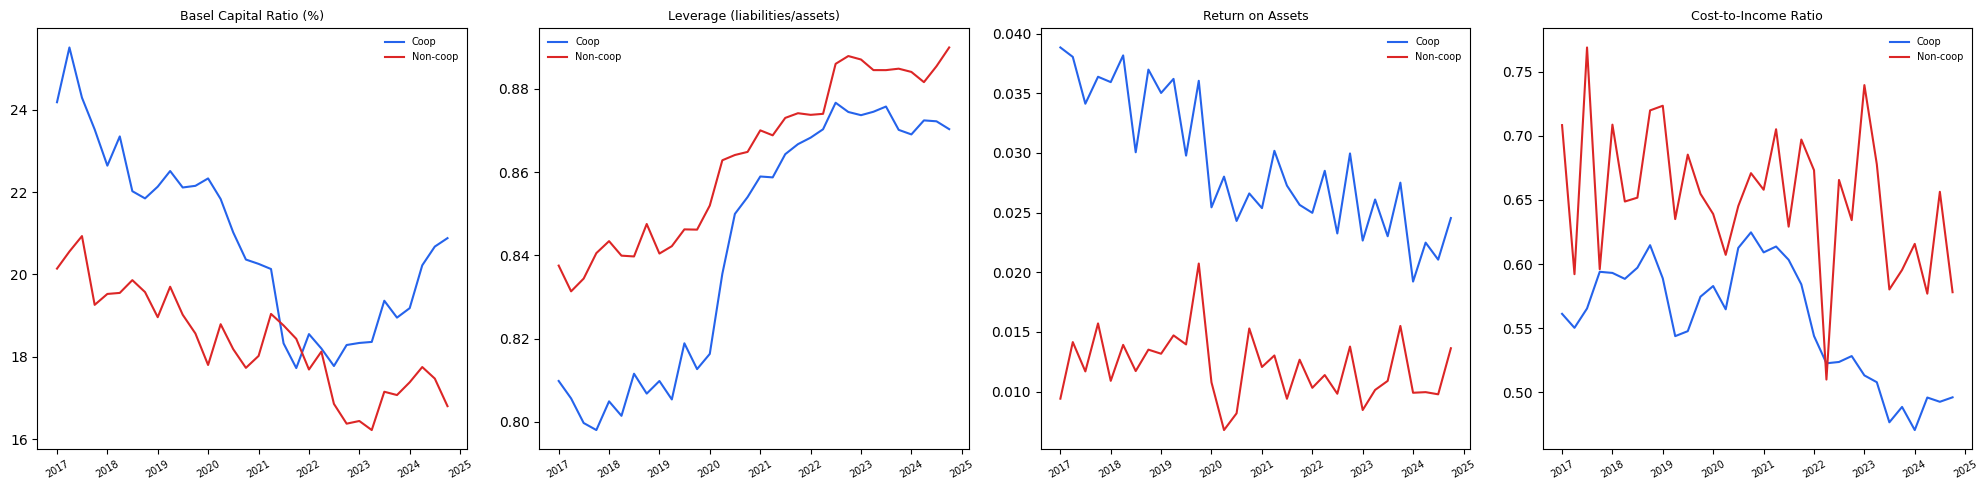
\includegraphics[width=\textwidth]{figures/fig11_stable.png}
\caption{Median values of four outcomes over the sample window, cooperatives and banks.
The cooperative median Basel ratio lies above the bank median for most of the window; the
negative differential in Table~\ref{tab:main} is a comparison at equal size. The
capital-conservation buffer was cut from 2.5 to 1.25 percent of risk-weighted assets in
April 2020 and restored in steps, to 1.625 percent in April 2021, 2.0 percent in October
2021 and 2.5 percent in April 2022 (Res.~4.783/2020), which lowered required, though not
reported, capital for all institutions; quarter fixed effects absorb this common shift.
Source: authors' calculations from BACEN IF.data.}
\label{fig:series}
\end{figure}

% =============================================================================
\section{Discussion}
% =============================================================================

The surviving results describe a focused retail lender. A cooperative in the
full-methodology population channels a high share of assets into member credit, runs that
operation at low cost, earns a solid return on assets without wide intermediation spreads, and sits in a narrow band
of the capital distribution rather than below it. This is consistent with a
member-service orientation in which capital accumulation is a means rather than an end
\citep{fonteyne2007}, and with the efficiency a focused retail model can deliver.

Our relation to \citet{hesse2007} is two parts in three. They find that cooperative banks
combine lower capitalisation, lower profitability and greater stability, with the
stability coming from lower return volatility. Lower capitalisation at comparable size and
lower return volatility both appear in our data. The profitability result does not:
cooperatives here earn more on assets, on margins indistinguishable from those of banks,
which points to cost discipline. In their sample stability is paid for with
profitability. In this population the two move together.

The combination that matters for supervision is capital and provisioning together, and the
distributional evidence changes what it says. At the thin end of the capital distribution,
where prudential concern would attach, cooperatives hold more capital than comparable banks,
and through most of the provisioning distribution they provision more. A
supervisory worry about thinly capitalised cooperatives running under-provisioned books is not
supported here. The data show the absence, among cooperatives, of the highly
capitalised upper tail that banks exhibit.

The pattern extends beyond capital.
Cooperatives are the more homogeneous group on every outcome we measure at equal size, and
several differentials that look large at the mean are differentials in dispersion. A
conditional mean is a poor summary of a comparison between a tight distribution and a diffuse
one, and reporting it alone describes the cooperative sector by reference to a region of the
bank distribution that cooperatives do not occupy.

Three analyst choices determined whether headline results existed. Defining the comparison
group as all non-cooperative institutions under the same methodology is the natural
regulatory reading of the population, and it imports nearly two hundred institutions that
hold no loans and take no deposits. Reading IF.data income fields as quarterly flows is
the natural reading of a quarterly file, and it mixes one- and two-quarter horizons. OLS
on a CEM-matched sample is the natural reading of matching plus regression, and it is not
the CEM estimand. None of these is exotic. Some of the literature's disagreements may
reflect different comparison groups.

\subsection{Limitations}

Five limitations bound the claims. Cooperative status is time-invariant, so the estimates
are conditional correlations and may reflect unobserved institutional characteristics
correlated with cooperative form. The full-methodology restriction selects the largest
cooperatives; Section~\ref{sec:selection} measures the resulting bias and finds it runs
toward zero for credit intensity and profitability and at most marginally away from zero
for efficiency, but the results generalise to that subpopulation. The provisioning ratio is an
accounting variable, not a measure of delinquency, so we report a null on provisioning
rather than a claim about credit risk. The stability outcomes are institution-level
statistics on a subsample of 105 cooperatives and 137 banks with at least eight
quarters, estimated without quarter effects, so they are less finely controlled than the
quarterly outcomes. Most systems are too thinly represented for separate
inference, and the independent segment cannot be assessed at all.

We also attempted a within-institution design and do not report one. The staggered movement
of cooperatives into the full methodology suggests a natural experiment. Adoption is driven
by growth, growth moves every balance-sheet ratio continuously, and pre-adoption trends run
through the adoption date rather than breaking at it. Matching adopters to non-adopters on
size and prior growth does not remove the trends. The threshold crossing does not identify
a regime effect in this setting.

% =============================================================================
\section{Contributions and Implications}
% =============================================================================

\subsection{Contributions}

We characterise cooperative behaviour under full Basel-style regulation in a large
emerging market, using the full population of full-methodology institutions,
with the regulatory environment fixed by construction. The substantive contribution is a
profile: credit-intensive, cost-efficient, profitable on assets, less volatile in
returns, and markedly more homogeneous than banks of the same size on every dimension we
measure. It comes with two nulls that correct
claims the same data appear to support under a looser comparison group.

We also supply a protocol. Define peers on the regulator's own categories, report a ladder
rather than a point, state how cumulative flows were converted to rates, report the matched
estimand rather than a matched-sample regression, and print treated cluster counts beside
system-level $p$-values. Each is cheap. In our data each changed a conclusion.

\subsection{Implications for proportional regulation}

Brazil's segmentation framework already applies proportionality along the size margin
\citep{cmn4553}. Our results speak to two further margins. We frame them as questions,
given the descriptive nature of the evidence.

The first is organisational architecture. The capital differential is concentrated in the
integrated systems, where centralised liquidity and consolidated risk management are
available, and the independent cooperatives, too few to measure, point the other way. A
proportional framework might recognise system membership, treating an integrated network
and its backstop as the relevant unit for parts of the capital and liquidity assessment,
rather than applying an individual-institution template uniformly. \citet{coelho2019}
report that several jurisdictions already do so.

The second is the calibration of the benchmark itself. A benchmark set against the average
full-methodology institution does not describe the cooperative configuration, because that
average is drawn from a distribution whose upper region cooperatives do not inhabit.
Cooperatives cluster in a narrow band of capitalisation, hold more capital than banks at the
thin end of the distribution, and provision at least as much. These are open questions. We
observe differences under a common methodology, and many institutional features other than
regulation differ between the two groups. The appropriate response is not necessarily
a lighter requirement. Section~\ref{sec:theory} indicates which way the finding cuts: the representation
rationale for the capital requirement as a stand-in for depositors too small and dispersed
to discipline the institution themselves weakens for a member-owned, network-monitored
cooperative, but the systemic-externality and public-guarantee rationales do not. Thinner
capital with no offsetting difference in provisioning bears on the rationales that do not
weaken, which is why it is a reason for supervisory attention as much as for relief.

For the cooperative movement, the difference does not vanish when the rules are equalised,
but it is narrower and more specific than an unexamined comparison suggests. A case resting
on cooperatives provisioning more conservatively than banks is not supported here. A case
resting on credit intensity, cost efficiency and return on assets is.

% =============================================================================
% Mudei a forma da bibliografia pra seguir o padrão pdflatex → bibtex → pdflatex → pdflatex. Aí não precisa colocar item a item da bibliografia. O latex ja puxa se tiver citado no texto.
\section{Key References}
% =============================================================================

\renewcommand{\refname}{}
\vspace{-2.5em}
\bibliographystyle{apalike}
\bibliography{references/references}

% =============================================================================
\appendix
\section{Reproducibility}
% =============================================================================

All results come from one script run against the public IF.data bulk files. The primary
specification is singular cooperatives (\texttt{b3S}) against banks (\texttt{b1},
\texttt{b2}) under full methodology, size-quintile coarsening, winsorisation within the
analysis sample, standard errors clustered by institution with wild cluster bootstrap
$p$-values from 1{,}999 replications. The broad and commercial comparison groups, the
region-exact coarsening, the unweighted matched regression, the winsorisation variants
and the conditional-median estimates are all parameters of the same function. The same
script writes the bootstrap $p$-values for every cell of the main table and the system
split, the winsorisation variants, the pre-adoption comparison of
Section~\ref{sec:selection}, the reverter and provisioning-coverage checks, and the
small-cluster simulation of Section~\ref{sec:inference} to a single robustness file.
Tables are generated from the results files rather than transcribed.

\end{document}